\chapter{Le détecteur Compact Muon Solenoid (CMS)}
\renewcommand\chapterillustration{CMS/cms.jpeg}
\ThisULCornerWallPaper{1}{\chapterillustration}
\minitoc

\lettrine[lines=4, slope=-0.5em]{C}{e} chapitre décrit le détecteur CMS et les sous-détecteurs qui le compose, suivi d'une discussion sur le système de déclenchement. Il décrit également certaines des mises à niveau qui se dérouleront durant les \textit{Long Shut Down} LS2 et LS3 afin de se préparer à l'augmentation de la luminosité et de l'empilement qui en découle.

\section{Le détecteur Solénoïde compact à muons (CMS)}
Le détecteur Solénoïde Compact à Muons abrégé en CMS (pour \textit{Compact Muon Solenoid}) est avec ATLAS une expérience généraliste qui a comme buts majeurs :

\begin{itemize}[label=$\bullet$]
	\item \textbf{La recherche du boson de Higgs : } Lors de la conception de CMS dans les années \num{1990}, la détection du boson de Higgs a été prise comme référence afin de tester les performances du design du détecteur. Ce but a été réalisé avec la découverte d'une particule compatible avec le boson de Higgs le \num{4} juillet \num{2012}.
	\item \textbf{Confirmer et préciser les mesures de la physique du Modèle Standard : } Des mesures de précisions dans des domaines tels que la QCD, le couplage électrofaible, et la physique des saveurs pourraient donner des indications d'une physique au-delà du Modèle Standard.
	\item \textbf{La recherche de signes de physique au-delà du Modèle Standard : }CMS permet la recherche de particules supersymétriques ou de nouveaux bosons vecteurs massifs ($Z'$) ou encore la recherche de dimensions supplémentaires par exemple.
	\item \textbf{Étudier les collisions d'ions lourds.}
\end{itemize}

Afin de répondre à ces objectifs, le "\textit{Technical Design Report}" (TDR) \cite{Bayatian:922757} a fixé le cahier des charges et les caractéristiques essentielles du détecteur CMS, à savoir :
\begin{itemize}[label=$\bullet$]
	\item Une bonne identification des muons et une bonne résolution en impulsion sur une vaste gamme d'impulsion pour la région $|\eta|<$\num{2.5}, une bonne résolution en masse pour les dimuons ($\approx$ \num{1}\% à \SI{100}{\giga\eV/\square\c}) et la capacité à déterminer de manière certaine la charge des muons d'impulsion $p<$ \SI{1}{\tera\eV/\c}.
	\item Une bonne résolution en impulsion pour les particules chargées ainsi qu'une bonne efficacité de reconstruction dans le trajectographe interne (\textit{inner tracker}). Un déclenchement et un étiquetage efficace pour les jets venant de quarks $\tau$ et $b$, ce qui requiert un détecteur à pixels proche du point d'interaction.
	\item Une bonne résolution pour l'énergie électromagnétique, et une bonne résolution en masse pour les diphotons et diélectrons  ($\approx$ \num{1}\% à \SI{100}{\giga\eV/\square\c}), une grande couverture géométrique ($|\eta|<2.5$), une mesure de la direction des photons et/ou une localisation correcte du vertex primaire d'interaction ainsi qu'une bon rejet des $\pi_{0}$ et une isolation des photons et leptons efficace à haute luminosité.
	\item une bonne résolution en masse des dijets et une bonne résolution en masse de l'énergie transverse manquante $E_{T}^{miss}$. Ceci requiert un calorimètre hadronique hermétique de très grande couverture géométrique ($|\eta|<5$) et une fine segmentation latérale ($\Delta\eta\times\Delta\phi<0.1\times0.1$)
\end{itemize} 

\subsection{Systèmes de coordonnées conventionnels}
Le système de coordonnées utilisé dans CMS est un repère cartésien $\left(O,\vec{x},\vec{y},\vec{z}\right)$ où $O$ est l'origine du repère et coïncide avec le point nominal d'interaction (IP) qui est le centre du détecteur. Le système de coordonnées est déterminé par l'axe $z$ qui est défini comme étant parallèle et dans la même direction que le faisceau allant dans le sens anti-horaire vue de dessus. L'axe $x$ pointe vers le centre du collisionneur LHC. L'axe $y$ est orthogonal au plan $xz$ et pointe vers le haut. CMS possédant une symétrie cylindrique, le repère $\left(O,\vec{r},\vec{\phi},\vec{z}\right)$ est souvent utilisé. $z$ correspond à la distance entre le plan perpendiculaire à l'axe du faisceau (appelé plan transverse) passant par le point considéré et l'origine $O$ du repère; $\phi$ est mesuré par rapport à l'axe $\vec{x}$ dans le plan $xy$ (angle d'émission par rapport à l'axe du faisceau) et $r=\sqrt{x^2+y^2}$. L'angle polaire $\theta$ est définit par rapport à $z$. Un troisième type de coordonnées, utilisant le fait que les particules produites au LHC sont relativistes, est également utilisé. En décomposant l'impulsion de la particule en une composante transverse et longitudinale $p=p_{T}+p_{L}=\sqrt{p_{x}^{2}+p_{y}^{2}}+p_{z}$ :
\begin{equation}
(E/c)^{2}=(mc)^{2}+p_{T}^{2}+p_{L}^{2}\Longrightarrow (E/c)^{2}-p_{L}^{2}=(mc)^{2}+p_{T}^{2}\Longrightarrow  \begin{cases}
\left(E/c \right)=\sqrt{\left(mc \right)^{2}+p_{T}^{2}}\cosh(y) \\
p_{L}=\sqrt{\left(mc \right)^{2}+p_{T}^{2}}\sinh(y)
\end{cases}
\end{equation}
%qu'il est possible de réécrire comme :
%\begin{equation}
%\left(E/c \right)=\sqrt{\left(mc \right)^{2}+p_{T}^{2}}\cosh(y), p_{L}=\sqrt{\left(mc \right)^{2}+p_{T}^{2}}\sinh(y)
%\end{equation}
avec $y$ un paramètre appelé rapidité. En remarquant que $p_{l}=p_{z}=p\cos(\theta)$ et en faisant le développement de $E=\sqrt{m^{2}c^{4}+p^{2}c^{2}}$:
\begin{equation}
y=\arctan\left(\frac{p_{l}c}{E}\right)=\frac{1}{2}\log\left(\frac{E+p_{l}c}{E-p_{l}c}\right)=\frac{1}{2}\log\left(\frac{\cos^2 \theta/2+\cdots}{\sin^2 \theta/2+\cdots}\right)\backsimeq-\log\tan\left(\frac{\theta}{2}\right)=\eta
\end{equation}
%en remarquant que $p_{l}=p_{z}=p\cos(\theta)$ et en faisant le développement de $E=\sqrt{m^{2}c^{4}+p^{2}c^{2}}$
%\begin{equation}
%y=\frac{1}{2} \log\left(\frac{E+p_{l}c}{E-p_{l}c}\right)=\frac{1}{2}\log\left(\frac{\cos^2 %\theta/2+m^{2}c^{2}/4p^{2}+\cdots}{\sin^2 %\theta/2+m^{2}c^{2}/4p^{2}+\cdots}\right)\backsimeq-\log\tan\left(\frac{\theta}{2}\right)=\eta
%\end{equation}
$\eta$ est appelé pseudo-rapidité. On utilise donc le repère $\left(O,\vec{r},\vec{\eta},\vec{\phi}\right)$ pour décrire la géométrie de CMS.

\subsection{Description générale de CMS}
Le détecteur CMS se trouve dans une caverne située au point \num{5} (P5) du LHC, proche du village de Cessy en France. La construction de CMS s'est effectuée en surface et par tranches autonomes afin de réduire le temps et les coûts nécessaires à sa construction.
\marginpar
{
	\centering
	\includegraphics[width=\marginparwidth]{CMS/slice.jpg}
	\captionof{figure}{Descente d'une tranche de CMS.}
	\label{slice}
}
Chaque tranche à ensuite été descendue dans la caverne et assemblée à \SI{100}{\meter} sous terre (cf.Fig~\ref{slice}).
CMS est une détecteur cylindrique de \SI{24}{\meter} de long et de \SI{14.6}{\meter} de diamètre pour une masse de plus de \num{16000} tonnes (cf.Fig~\ref{cmsexploded}). Il est composé d'une succession de sous-détecteurs concentriques.

\begin{sidewaysfigure}
	\centering
	\includegraphics[width=0.80\textwidth]{CMS/cms.png}
	\caption{\label{cmsexploded}Vue éclatée du détecteur CMS.}
\end{sidewaysfigure}
\newpage
En partant du centre vers l'extérieur :
\begin{itemize}[label=$\bullet$]
	\item \textbf{Le trajectographe : } C'est le sous-détecteur le plus proche du point d'interaction. Il permet de reconstruire la trajectoires des particules chargées.
	 \item \textbf{Le calorimètre électromagnétique (ECAL\footnote{Pour \textit{Electromagnetic CALorimeter}.})}: Il permet de mesurer l'énergie des photons et des électrons.
	 \item \textbf{Le calorimètre hadronique (HCAL\footnote{Pour \textit{Hadronic CALorimeter}.})}: Il permet de mesurer l'énergie des hadrons.
	 \item \textbf{L'aimant supra-conducteur : } Il produit un champ de \SI{3.8}{\tesla} et permet de courber la trajectoire des particules chargées.
	 \item \textbf{Les chambres à muons : } Elles permettent d'identifier, reconstruire la trajectoire et mesurer l'énergie des muons. 
\end{itemize}
Chaque composant de CMS fera l'objet d'une description plus détaillée dans les paragraphes suivants.

\section{Les sous-détecteurs de CMS}
\subsection{Le trajectographe}
Le trajectographe de CMS (cf.Fig~\ref{trajectographe}) est le détecteur le plus proche du faisceau et du point de collision. Le trajectographe est composé de deux sous-détecteurs : le détecteur à pixels et le trajectographe à micro-pistes de silicium. Il a pour but de reconstruire les traces des particules chargées issues des collisions grâce à des suites d'impacts enregistrés par les couches du détecteur. La trace reconstruite permet de déterminer la charge et l'impulsion de la particule associée. En effet, une particule de charge $q$ qui se déplace dans un champ magnétique subit une force donné par la formule de \bsc{Lorentz}. La trajectoire de la particule dans le cas d'un champ magnétique d'intensité $B$ est hélicoïdale, de rayon $R_{c}$. Il est ainsi possible dans déduire l'impulsion transverse :
\begin{equation}
p_{T}=qBR_{c}
\end{equation}
En prenant les positions selon $r$ des hits, il est possible d'en déduire l'angle $\theta$, angle entre la trajectoire de la particule est le faisceau et donc de calculer l'impulsion totale:
\begin{equation}
p=\frac{p_{T}}{\sin\theta}
\end{equation}
\begin{figure}[ht!]
	\centering
	\includegraphics[width=0.65\textwidth]{CMS/tracker.png}
	\captionof{figure}{Schéma du trajectographe de CMS. Chaque trait représente un module du détecteur. Les lignes doubles correspondent à des modules mis dos à dos produisant des hits dit "stéréos". Le détecteur à pistes est composé de quatre sous-détecteurs : Les tonneaux internes (TIB), les tonneaux externes (TOB), les disques internes (TID) et les bouchons (TEC).}
	\label{trajectographe}
\end{figure}

\subsubsection{Le détecteur à pixels}
Le détecteur à pixels de CMS a récemment été remplacé afin de garder une trajectographie performante à des luminosités au dessus de \SI{2e34}{\per\square\centi\meter\per\second} et avec un empilement de plus de \num{50}. Ce remplacement a eu lieu du \num{28} février au \num{7} mars \num{2017} durant l'arrêt technique hivernal prolongé (EYETS). Le nouveau détecteur à pixels se compose d'un tonneau constitué de quatre couches de détection (BPIX) à des distances du faisceau $r=\SI{3.0}{\centi\meter}$, \SI{6.8}{\centi\meter}, \SI{10.2}{\centi\meter} et \SI{16}{\centi\meter} et d'une longueur de \SI{548.8}{\milli\meter} et de trois bouchons (FPIX) situé à $\pm$\SI{29.1}{\centi\meter}, $\pm$\SI{39.6}{\centi\meter} et $\pm$\SI{51.6}{\centi\meter} pour une couverture radiale allant de \num{4.5} à \SI{16.1}{\centi\meter}. Une comparaison entre l'ancien détecteur à pixel et le nouveau est donnée figure \ref{pixel}.

	\begin{figure}[ht!]
	\subfloat[Vue oblique-transverse comparant les couches des tonneaux de l'ancien (gauche) et du nouveau détecteur (droite).]{\includegraphics[width=.45\linewidth]{CMS/pixel.png}}
	\hfill
	\subfloat[Ancien détecteur à pixel (bas) et nouveau (haut).]{\includegraphics[width=.45\linewidth]{CMS/pixel2.png}}
	\caption{Comparaison entre le nouveau et l'ancien trajectographe à pixels.}
	\label{pixel}
\end{figure}

L'ajout d'une quatrième couche de détection dans le barrel assure une redondance lors de la reconnaissance de motifs et permet de réduire le taux d'erreurs lors d'empilement importants. Il assure également une sécurité au cas où la couche la plus proche du point d'interaction viendrait à se détériorer plus vite que prévu. Cependant, elle augmente le budget matière du détecteur, il a donc été nécessaire de repenser le support et les services afin d'être plus léger. Un nouveau système de refroidissement au \chemform{CO_2} ainsi que le déplacement des systèmes passifs (connectique, plaques d'électronique) hors du volume de trajectographie ont également été effectués (cf.Fig~\ref{pixel2}).

\begin{figure}[ht!]
	\centering
	\includegraphics[width=0.75\textwidth]{CMS/pixel3.png}
	\captionof{figure}{Vue explosée du nouveau détecteur à pixels. La figure montre les positions des différentes partitions FPIX et BPIX ainsi que leurs cylindres contenant leurs services respectifs. Les services nécessaires au détecteur (connectiques, fibres optiques, convertisseurs DC-DC sont situés à haut $\eta$, hors du volume de trajectographie).}
	\label{pixel2}
\end{figure}

Ce détecteur contient plus de \num{97} millions de pixels (\num{79} pour les BPIX et \num{18} pour les FPIX) mesurant \num{100}$\times$\SI{150}{\square\micro\meter} de section et \SI{250}{\micro\meter} d'épaisseur. Ces pixels sont regroupés en modules (\num{1184} pour BPIX et \num{672} pour FPIX) (cf.Fig~\ref{module}) de \num{66560} pixels  (\num{8}$\times$\num{2} ROCs) d'une épaisseur de \SI{75}{\micro\meter} pour la première couche du BPIX et \SI{250}{\micro\meter} pour le reste du BPIX et FPIX.

	\begin{figure}[ht!]
	\centering
	\subfloat[Module pour les couches \num{2} à \num{4} des BPIX et des FPIX (gauche) et de la couche \num{1} de BPIX (droite).]{\includegraphics[width=.46\linewidth]{CMS/module.png}}
	\hfill
	\subfloat[Schéma de l'électronique de lecture d'un module.]{\includegraphics[width=.46\linewidth]{CMS/module2.png}}
	\caption{Modules de pixels.}
	\label{module}
\end{figure}
\subsubsection{Le détecteur à pistes}
Le détecteur à pistes mesure \SI{5.5}{\meter} de long pour \SI{2.4}{\meter} de diamètre pour une aire active de \SI{198}{\square\meter} et est le plus grand détecteur au silicium jamais construit. Il comporte en tout \num{15148} modules pour un total de \num{9.3} millions de pistes lues par \num{76000} puces électroniques. Il peut être décomposé en quatre sous-détecteurs :

\begin{itemize}[label=$\bullet$]
\item \textbf{Le tonneau interne} (TIB) (cf.Fig~\ref{TIB}) pour  \textit{Tracker Inner Barrel} est composé de \num{2724} modules répartis en quatre couches. Chaque couche se compose de pistes de silicium d'une épaisseur de \SI{320}{\micro\meter} avec un pas de \SI{80}{\micro\meter} pour les deux premières couches et de \SI{120}{\micro\meter} pour les deux dernières. Elles sont orientées parallèlement au faisceau. Les deux premières couches sont composées de modules dits "stéréos" qui sont la juxtaposition de deux modules collés l'un l'autre avec un angle de \SI{100}{\milli\radian} entre les deux, ce qui permet d'avoir une résolution de \num{23} à \SI{34}{\micro\m} dans le plan transverse et de \SI{230}{\micro\meter} dans le plan longitudinal. Son rayon est compris entre \num{25} et \SI{52}{\centi\meter} et sa longueur couvre le domaine $|z|<$\SI{65}{\centi\meter}.

\item \textbf{Les disques internes} (TID) (cf.Fig~\ref{TID}) pour \textit{Tracker Inner Disk} sont composés de trois disques parallèles qui sont compris dans le domaine \SI{75}{\centi\meter}$<|z|<$\SI{110}{\centi\meter}. Chaque disque est composé de trois anneaux concentriques. Les \num{816} modules sont composés de strips d'une épaisseur de \SI{320}{\micro\meter} orientés radialement pour un pas compris entre \SI{81} et \SI{158}{\micro\meter}. Comme pour le TIB, les deux premiers modules sont "stéréos".
\marginpar
{
	\centering
	\includegraphics[width=\marginparwidth]{CMS/TOB_TEC.png}
	\captionof{figure}{Différents modules utilisés pour la construction du TOB et du TEC.}
	\label{TOB_TEC}
}
\item \textbf{Le tonneau externe } (TOB) (cf.Fig~\ref{TOB}) pour \textit{Tracker Outer Barrel} entoure les TIB et TID pour couvrir un espace entre \num{60} et \SI{100}{\centi\meter} en rayon et $|z|<$\SI{110}{\centi\meter}. Il est composé de \num{5208} modules (cf.Fig~\ref{TOB_TEC}) de pistes orientées parallèlement aux faisceaux et de pas compris entre \num{122} et \SI{183}{\micro\meter}. Ces modules sont répartis en six couches dont les deux dernières sont "stéréos". L'épaisseur de ces modules est de \SI{500}{\micro\meter}.   

\item \textbf{Les bouchons }(TEC) (cf.Fig~\ref{TEC}) pour \textit{Tracker End-Cap} sont composés de neuf disques chacun, de \num{4} à \num{7} anneaux concentriques. Ils couvrent \num{25}--\SI{110}{\centi\meter} en rayons et \num{120}--\SI{275}{\centi\meter} en $|z|$. Les deux premiers disques ainsi que le cinquième sont "stéréos". Les trois premiers anneaux sont composés de \num{1256} modules par bouchon (cf.Fig~\ref{TOB_TEC}) d'épaisseur \SI{320}{\micro\meter} et de pas inter-pistes compris entre \num{81} et \SI{158}{\micro\meter}. Les quatre anneaux suivant, sont composés de \num{1944} modules par bouchon (cf.Fig~\ref{TOB_TEC}), d'épaisseur \SI{500}{\micro\meter} de pas inter-strip \num{113}--\SI{172}{\micro\meter}.
\end{itemize}

	\begin{figure}[ht!]
	\centering
	\subfloat[Le TIB.]{\includegraphics[width=.40\linewidth]{CMS/TIB.jpg}\label{TIB}}
	\subfloat[Un TID.]{\includegraphics[width=.40\linewidth]{CMS/TID.jpg}\label{TID}}
	\\
	\subfloat[Le TOB.]{\includegraphics[width=.40\linewidth]{CMS/TOB.jpg}\label{TOB}}
	\subfloat[Un TEC.]{\includegraphics[width=.40\linewidth]{CMS/TEC.jpg}\label{TEC}}
	\caption{Photos des différents composants du détecteur à pistes.}
\end{figure}

\newpage
\subsection{Le calorimètre électromagnétique}
Le calorimètre électromagnétique de CMS ou \textit{Electromagnetic CALorimeter} (ECAL), permet de mesurer l'énergie et la direction des particules réagissant principalement à l'interaction électromagnétique. Ce sont surtout les photons et les électrons qui seront détectés; ils perdent leur énergie par des processus radiatifs. La distance caractéristique est donnée par la longueur de radiation $X_{0}$, dépendante du matériau, définie comme le libre parcours moyen pour le processus de radiation. Des photons de \SI{100}{\giga\eV} perdent à peu près toute leur énergie dans \num{20}$\times X_{0}$.
\begin{figure}[ht!]
	\centering
	\includegraphics[width=0.90\textwidth]{CMS/ECAL.png}
	\captionof{figure}{Schéma du ECAL de CMS.}
	\label{ECAL}
\end{figure}

Le calorimètre électromagnétique est composé de \num{75848} cristaux (cf.Fig~\ref{crystaux}) de \chemform{PbWO_4} (\SI{11}{\cubic\meter}, \num{92} tonnes) et peut se décomposer en trois sous-structures (cf.Fig~\ref{ECAL}) :
\begin{itemize}[label=$\bullet$]
	\item \textbf{Le tonneau} ou EB (cf.Fig~\ref{EB}) pour \textit{Electromagnetic Barrel} contient \num{61200} cristaux de tungstate de plomb. Le tonneau est divisé en \num{36} supermodules couvrant chacun la moitié de la longueur du tonneau. Chaque super-module contient \num{1700} cristaux de \num{22}$\times$\SI{22}{\square\milli\meter} et de longueur \SI{230}{\milli\meter}. Les cristaux sont arrangés de manière à former \num{170}-$\eta$ anneaux contenant \num{360} cristaux chacun. Un cristal couvre environ \SI{1}{\degree} en $\phi$. Le tonneau couvre une zone en pseudorapidité de $|\eta|<$\num{1.479}. Les photodiodes à avalanche (cf.Fig~\ref{APD}) (APD) sont utilisées pour détecter la scintillation.
	\marginpar
	{
		\centering
		\includegraphics[width=\marginparwidth]{CMS/Crystaux.png}
		\captionof{figure}{Un cristal de \chemform{PbWO_4}.}
		\label{crystaux}
	}
	
	\marginpar
	{
		\centering
		\includegraphics[width=\marginparwidth]{CMS/APD.png}
		\captionof{figure}{Un groupe de deux APD.}
		\label{APD}
	}
	\marginpar
	{
		\centering
		\includegraphics[width=\marginparwidth]{CMS/dee.jpg}
		\captionof{figure}{Un \textit{"Dee"}.}
		\label{DEE}
	}
	\marginpar
	{
		\centering
		\includegraphics[width=\marginparwidth]{CMS/20SCs.jpg}
		\captionof{figure}{Montage de \num{20} Super-Cristaux sur un des \textit{Dee}.}
		\label{SP}
	}
	\marginpar
	{
		\centering
		\includegraphics[width=\marginparwidth]{CMS/VPT.png}
		\captionof{figure}{Une VPT.}
		\label{VPT}
	}
	
	\item \textbf{Les bouchons} (EE) (cf.Fig~\ref{EE}) pour \textit{Electromagnetic End-cap} sont perpendiculaires aux faisceaux et ferment le EB. Ils sont situés à \SI{315}{\centi\meter} du point d'interaction et couvrent une section en $\eta$ allant de \num{1.479} à \num{3}. Chaque bouchon se décompose en deux demi-disques appelés \textit{"Dee"} (cf.Fig~\ref{DEE}). Chaque \textit{Dee} est constitué de \num{3662} cristaux de \num{2.86}$\times$\SI{2.86}{\centi\meter} et de longueur \SI{220}{\milli\meter} regroupés en matrices de \num{5}$\times$\num{5} qu'on appelle Super-Cristaux (cf.Fig~\ref{SP}). La scintillation est détectée par des phototriodes à vide (VPT) (cf.Fig~\ref{VPT}). Les cristaux de \chemform{PbWO_4} ont une grande densité ($\rho=$\SI{8.28}{\gram\per\cubic\centi\meter}), une longueur d'interaction $X_{0}$ assez courte de \SI{0.89}{\centi\meter} est un petit rayon de Molière ($r_{M}=$\SI{2.2}{\centi\meter}) ainsi qu'une grande vitesse de radiation (\num{80}\% dans \SI{25}{\nano\second}). 
	\item \textbf{L'initiateur de gerbe } (cf.Fig~\ref{PRESHOWER}), appelé \textit{Preshower} est placé entre le EB et le EE. Il consiste en deux couches de détecteurs de silicium de pas \SI{1.9}{\milli\meter} intercalées entre deux couches en plomb (\num{2}$X_{0}$ devant et \num{1}$X_{0}$ derrière la première couche de silicium). Il permet d'améliorer la précision de la mesure de la position de la gerbe électromagnétique et la discrimination $\gamma/\pi_{0}$. Il couvre une région comprise entre \num{1.653}$<|\eta|<$\num{2.6}.
\end{itemize}
\begin{figure}[ht!]
	\centering
	\subfloat[Le tonneau du ECAL (EB).]{\includegraphics[width=0.8\linewidth]{CMS/EB.jpg}\label{EB}}
	\\
	\subfloat[Un bouchon du ECAL (EE).]{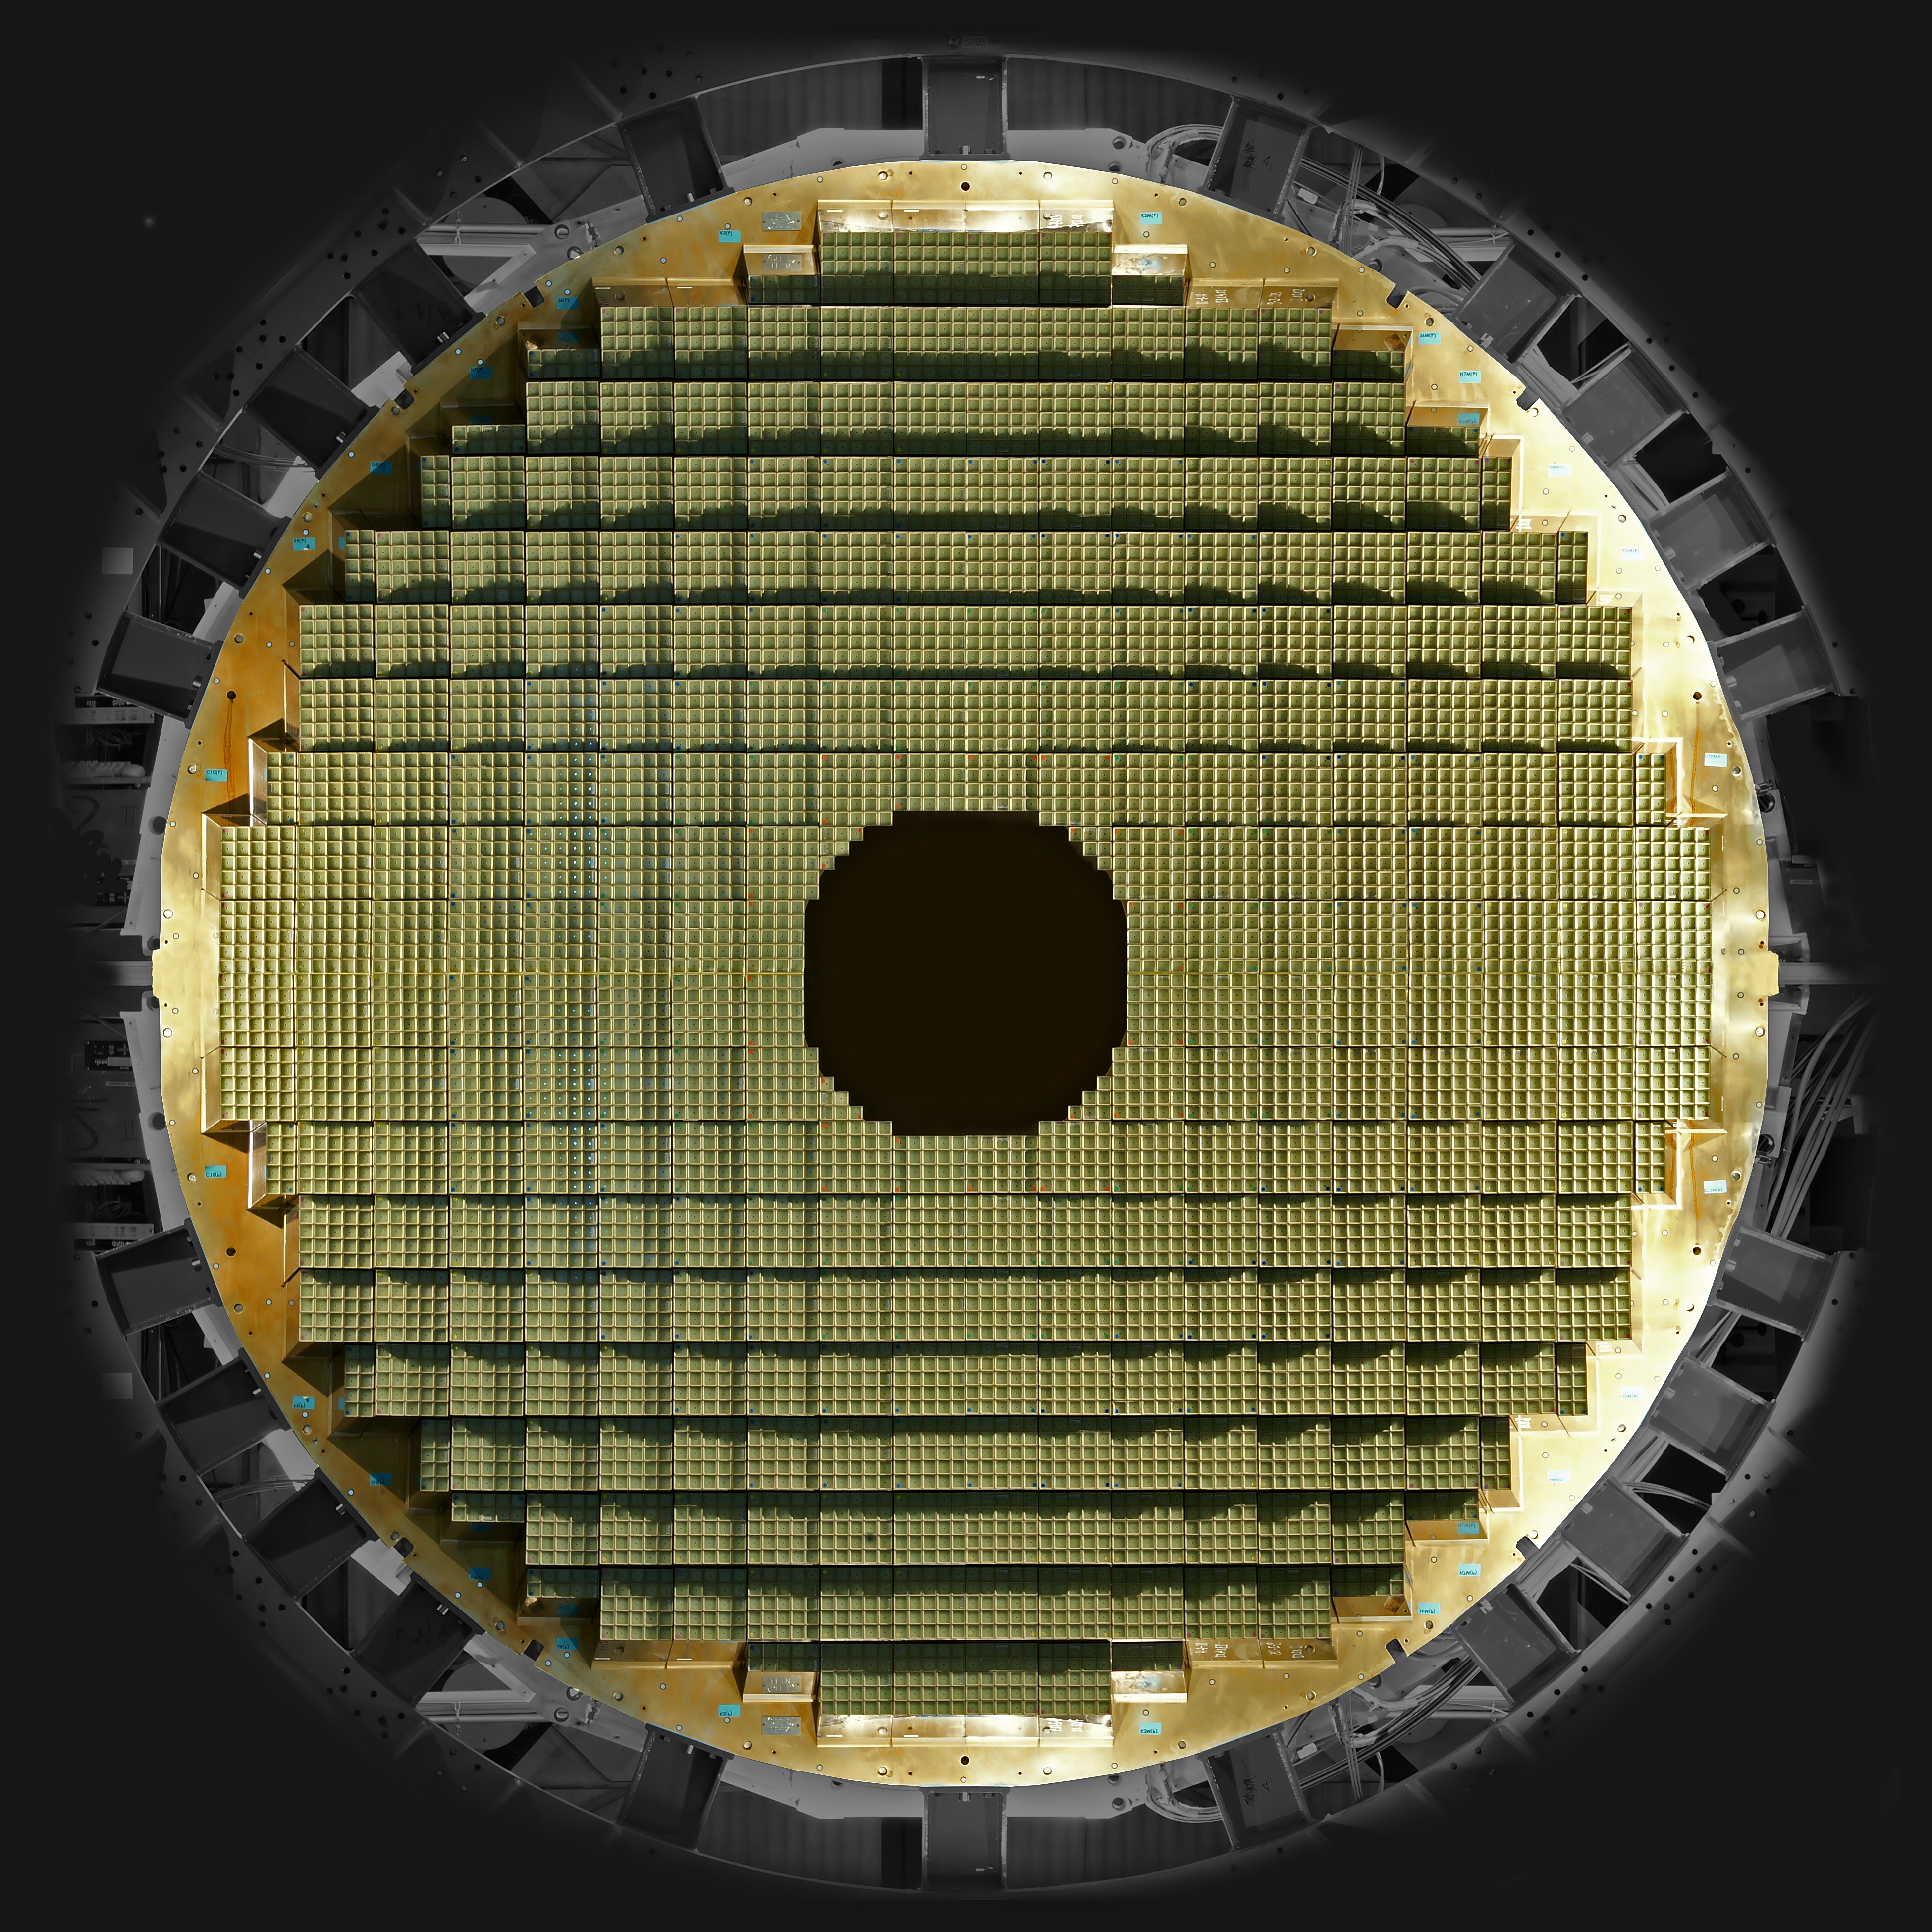
\includegraphics[width=.40\linewidth]{CMS/EE.jpg}\label{EE}}
	\subfloat[Un des preshower du ECAL.]{\includegraphics[width=.40\linewidth]{CMS/preshower.jpg}\label{PRESHOWER}}
	\caption{Photos des différents composants du calorimètre électromagnétique.}
\end{figure}
\subsection{Le calorimètre hadronique}
	\marginpar
{
	\centering
	\includegraphics[width=\marginparwidth]{CMS/LAITON.jpg}
	\captionof{figure}{Photo de douilles de la marine russe réutilisées pour la construction du HCAL.}
	\label{LAITON}
}
	\marginpar
{
	\centering
	\includegraphics[width=\marginparwidth]{CMS/SCINTI.png}
	\captionof{figure}{Photo d'une tuile du HO avec des fibres WLS insérées dans les \num{4} $\sigma$-rainures.}
	\label{SCINTI}
}
\marginpar
{
	\centering
	\includegraphics[width=\marginparwidth]{CMS/MPPC.png}
	\captionof{figure}{Photo d'un MPPC.}
	\label{MPPC}
}
\marginpar
{
	\centering
	\includegraphics[width=\marginparwidth]{CMS/HPD.png}
	\captionof{figure}{Photo d'une HPD.}
	\label{HPD}
}
Le calorimètre hadronique de CMS ou \textit{Hadronic CALorimeter} (HCAL) (cf.Fig~\ref{HCAL}) permet de mesurer l'énergie et la direction des hadrons issus de l'hadronisation des quarks et gluons produits lors des collisions. Ce détecteur à une grande compacité spatiale et énergétique et est très compact car il se trouve pour une grande partie entre le ECAL et l'aimant supraconducteur. Cette disposition a nécessité de maximiser la quantité d'absorbeur et de minimiser les parties actives du détecteur. L'absorbeur est constitué de laiton (cf.Fig~\ref{LAITON}) qui possède une faible longueur d'interaction $\lambda_{l}$ et un faible taux de diffusions multiples. Les hadrons perdent majoritairement leur énergie par interaction nucléaire avec l'absorbeur. La plupart des hadrons sont stoppés avec \num{9}$\lambda_{l}$. Le laiton est également non magnétique ce qui est nécessaire vu l'emplacement du calorimètre. Le matériau actif est composé de feuilles de scintillateurs fluorescents (cf.Fig~\ref{SCINTI}). La scintillation est ensuite récoltée par des fibres optiques qui décalent la longueur d'onde de la lumière (WLS). Le signal est ensuite lu par des \textit{Multi-Pixel Photon Counter} (MPPC) (cf.Fig~\ref{MPPC}) pour le sous-détecteur \textit{Hadronic Outward calorimeter} et par des photodiodes hybrides (HPD) (cf.Fig~\ref{HPD}) pour les autres sous-détecteurs.
\begin{figure}[ht!]
	\centering
	\includegraphics[width=0.95\textwidth]{CMS/HCALSCHEME.png}
	\captionof{figure}{Schéma d'un quart d'une coupe du HCAL de CMS.}
	\label{HCAL}
\end{figure}

Le calorimètre hadronique couvre une zone en pseudo-rapidité jusqu'à $|\eta|<$\num{5.0}. Il possède plus de \num{70000} feuilles de scintillateurs. Il est composé de \num{4} sous-détecteurs subdivisés en tours : 
\begin{itemize}[label=$\bullet$]
	\item \textbf{Le tonneau} HB pour \textit{Hadronic Barrel calorimeter} (cf.Fig~\ref{HB}) couvre la région en pseudo rapidité $|\eta|<1.3$. Il est constitué de \num{36} quartiers couvrant \SI{20}{\degree} en $\phi$ découpés en quatre sous secteurs de \SI{5}{\degree} en $\phi$ et \num{16} sous secteurs en $\eta$. Un quartier possède \num{16} couches qui sont des empilements de scintillateurs de \SI{9}{\milli\meter} d'épaisseur pour les couches les plus externes et \SI{3.7}{\milli\meter} pour les autres et d'absorbeur de (\SI{40}{\milli\meter} de fer pour la première couche, \SI{50.5}{\milli\meter} de laiton pour les huit suivantes, \SI{56.5}{\milli\meter} de laiton pour les six suivantes et \SI{75}{\milli\meter} de fer pour la dernière). Les tours ont une segmentation de $\Delta\eta\times\Delta\phi=$\num{0.087}$\times$\num{0.087}.
	\item \textbf{Les deux bouchons} HE pour \textit{Hadronic End-cap calorimeter} (cf.Fig~\ref{HE}) couvrent les régions comprises entre $|\eta|>$\num{1.3} et $|\eta|<$\num{3.0}. Une zone inclinée à \SI{53}{\degree} par rapport à l'axe du faisceau et ne pointant pas vers le point d'interaction est laissée libre afin de permettre le passage des câbles et systèmes nécessaires au trajectographe et au calorimètre électromagnétique. Les bouchons sont segmentés en \num{18} quartiers de \SI{20}{\degree} en $\phi$ chacun composé de \num{14} tours en $\eta$. Les tours sont des empilements de scintillateurs de \SI{3.7}{\milli\meter} d'épaisseur et d'une couche d'absorbeur (\SI{9}{\milli\meter} pour la première couche et \SI{7.5}{\milli\meter} pour les suivantes). Une tour possède \num{19} couches de  scintillateurs en tout. Les \num{5} tours couvrant $|\eta|<$\num{1.74} ont une segmentation de $\Delta\eta\times\Delta\phi=$\num{0.087}$\times$\num{0.087} alors que les \num{8} couvrant \num{1.74}$<|\eta|<$\num{3.0} ont des segmentations allant de $\Delta\eta\times\Delta\phi=$\num{0.09}$\times$\num{0.174} à $\Delta\eta\times\Delta\phi=$\num{0.35}$\times$\num{0.174}.
	\item \textbf{Le calorimètre externe} HO pour \textit{Hadronic Outward calorimeter} (cf.Fig~\ref{HO}) est placé à l'extérieur de l'aimant supraconducteur. Il est constitué de couches de scintillateurs de \SI{10}{\milli\meter} d'épaisseur et couvre la région $|\eta|<$\num{1.26}. Ce sous-détecteur permet de récupérer l'énergie sortant du HB et assure une longueur d'interaction de plus de \num{10}$\lambda_{l}$. Le HO est composé de \num{5} anneaux de \SI{2.536}{\meter} de long selon $z$ numérotés $-$\num{2}, $-$\num{1}, \num{0}, $+$\num{1}, $+$\num{2} et de centre $z=-$\num{5.324}, \num{2.686}, \num{0}, \num{2.686} et \SI{5.324}{\meter} respectivement. Le premier anneau est composé de deux couches de scintillateurs de \SI{10}{\milli\meter} d'épaisseur placées en $r=$\SI{3.82}{\meter} et \SI{4.07}{\meter}. Les autres anneaux ne possèdent qu'une couche de scintillateur placé à $r=$\SI{4.07}{\meter}. Chaque anneau est segmenté en \num{12} secteurs en $\phi$. Chaque secteur est segmenté en \num{8}, \num{6} et \num{5} tuiles de scintillateurs (cf.Fig~\ref{SCINTI}) pour les anneaux \num{0}, $\pm$\num{1}, $\pm$\num{2} respectivement.
	\item \textbf{Les calorimètres très à l'avant} HF pour \textit{Hadronic Forward calorimeter} couvrent une zone en pseudo-rapidité comprise entre $|\eta|>$\num{3.0} et $|\eta|<$\num{5.0} et \SI{12.5}{\centi\meter}$<r<$\SI{130}{\centi\meter}. Ils sont situés à une distance $|z|=$\SI{11.2}{\meter} et font \SI{1.65}{\meter} de long. Ils consistent en un absorbeur de fer qui intègre des fibres de quarks résistantes aux radiations qui assurent la collection rapide de la lumière \bsc{Čerenkov}. La moitié de ces fibres font toute la longueur du détecteur (\SI{1.65}{\meter}) alors que d'autres commencent à \SI{22}{\centi\meter} (soit \SI{143}{\centi\meter} de long) du bord placées vers l'intérieur de CMS. Elles sont placées alternativement à une distance de \SI{5}{\milli\meter} l'une de l'autre en $r$  avec segmentation de $\Delta\eta\times\Delta\phi=$\num{0.175}$\times$\num{0.175}. Cette différence de longueur permet de séparer les cascades électromagnétiques des cascades hadroniques. La lumière est ensuite collectée par des tubes photo-multiplicateurs (PMT). Le HF est composé de \num{18} secteurs de \SI{20}{\degree} en $\phi$. Chaque secteur comporte \num{13} anneaux en $\eta$.
\end{itemize}
\begin{figure}[ht!]
\centering
\subfloat[Le tonneau du HCAL (HB).]{\includegraphics[width=.40\linewidth]{CMS/HB.jpg}\label{HB}}
\subfloat[Un bouchon du HCAL (HE).]{\includegraphics[width=.40\linewidth]{CMS/HE.jpg}\label{HE}}
\\
\subfloat[Installation du HO.]{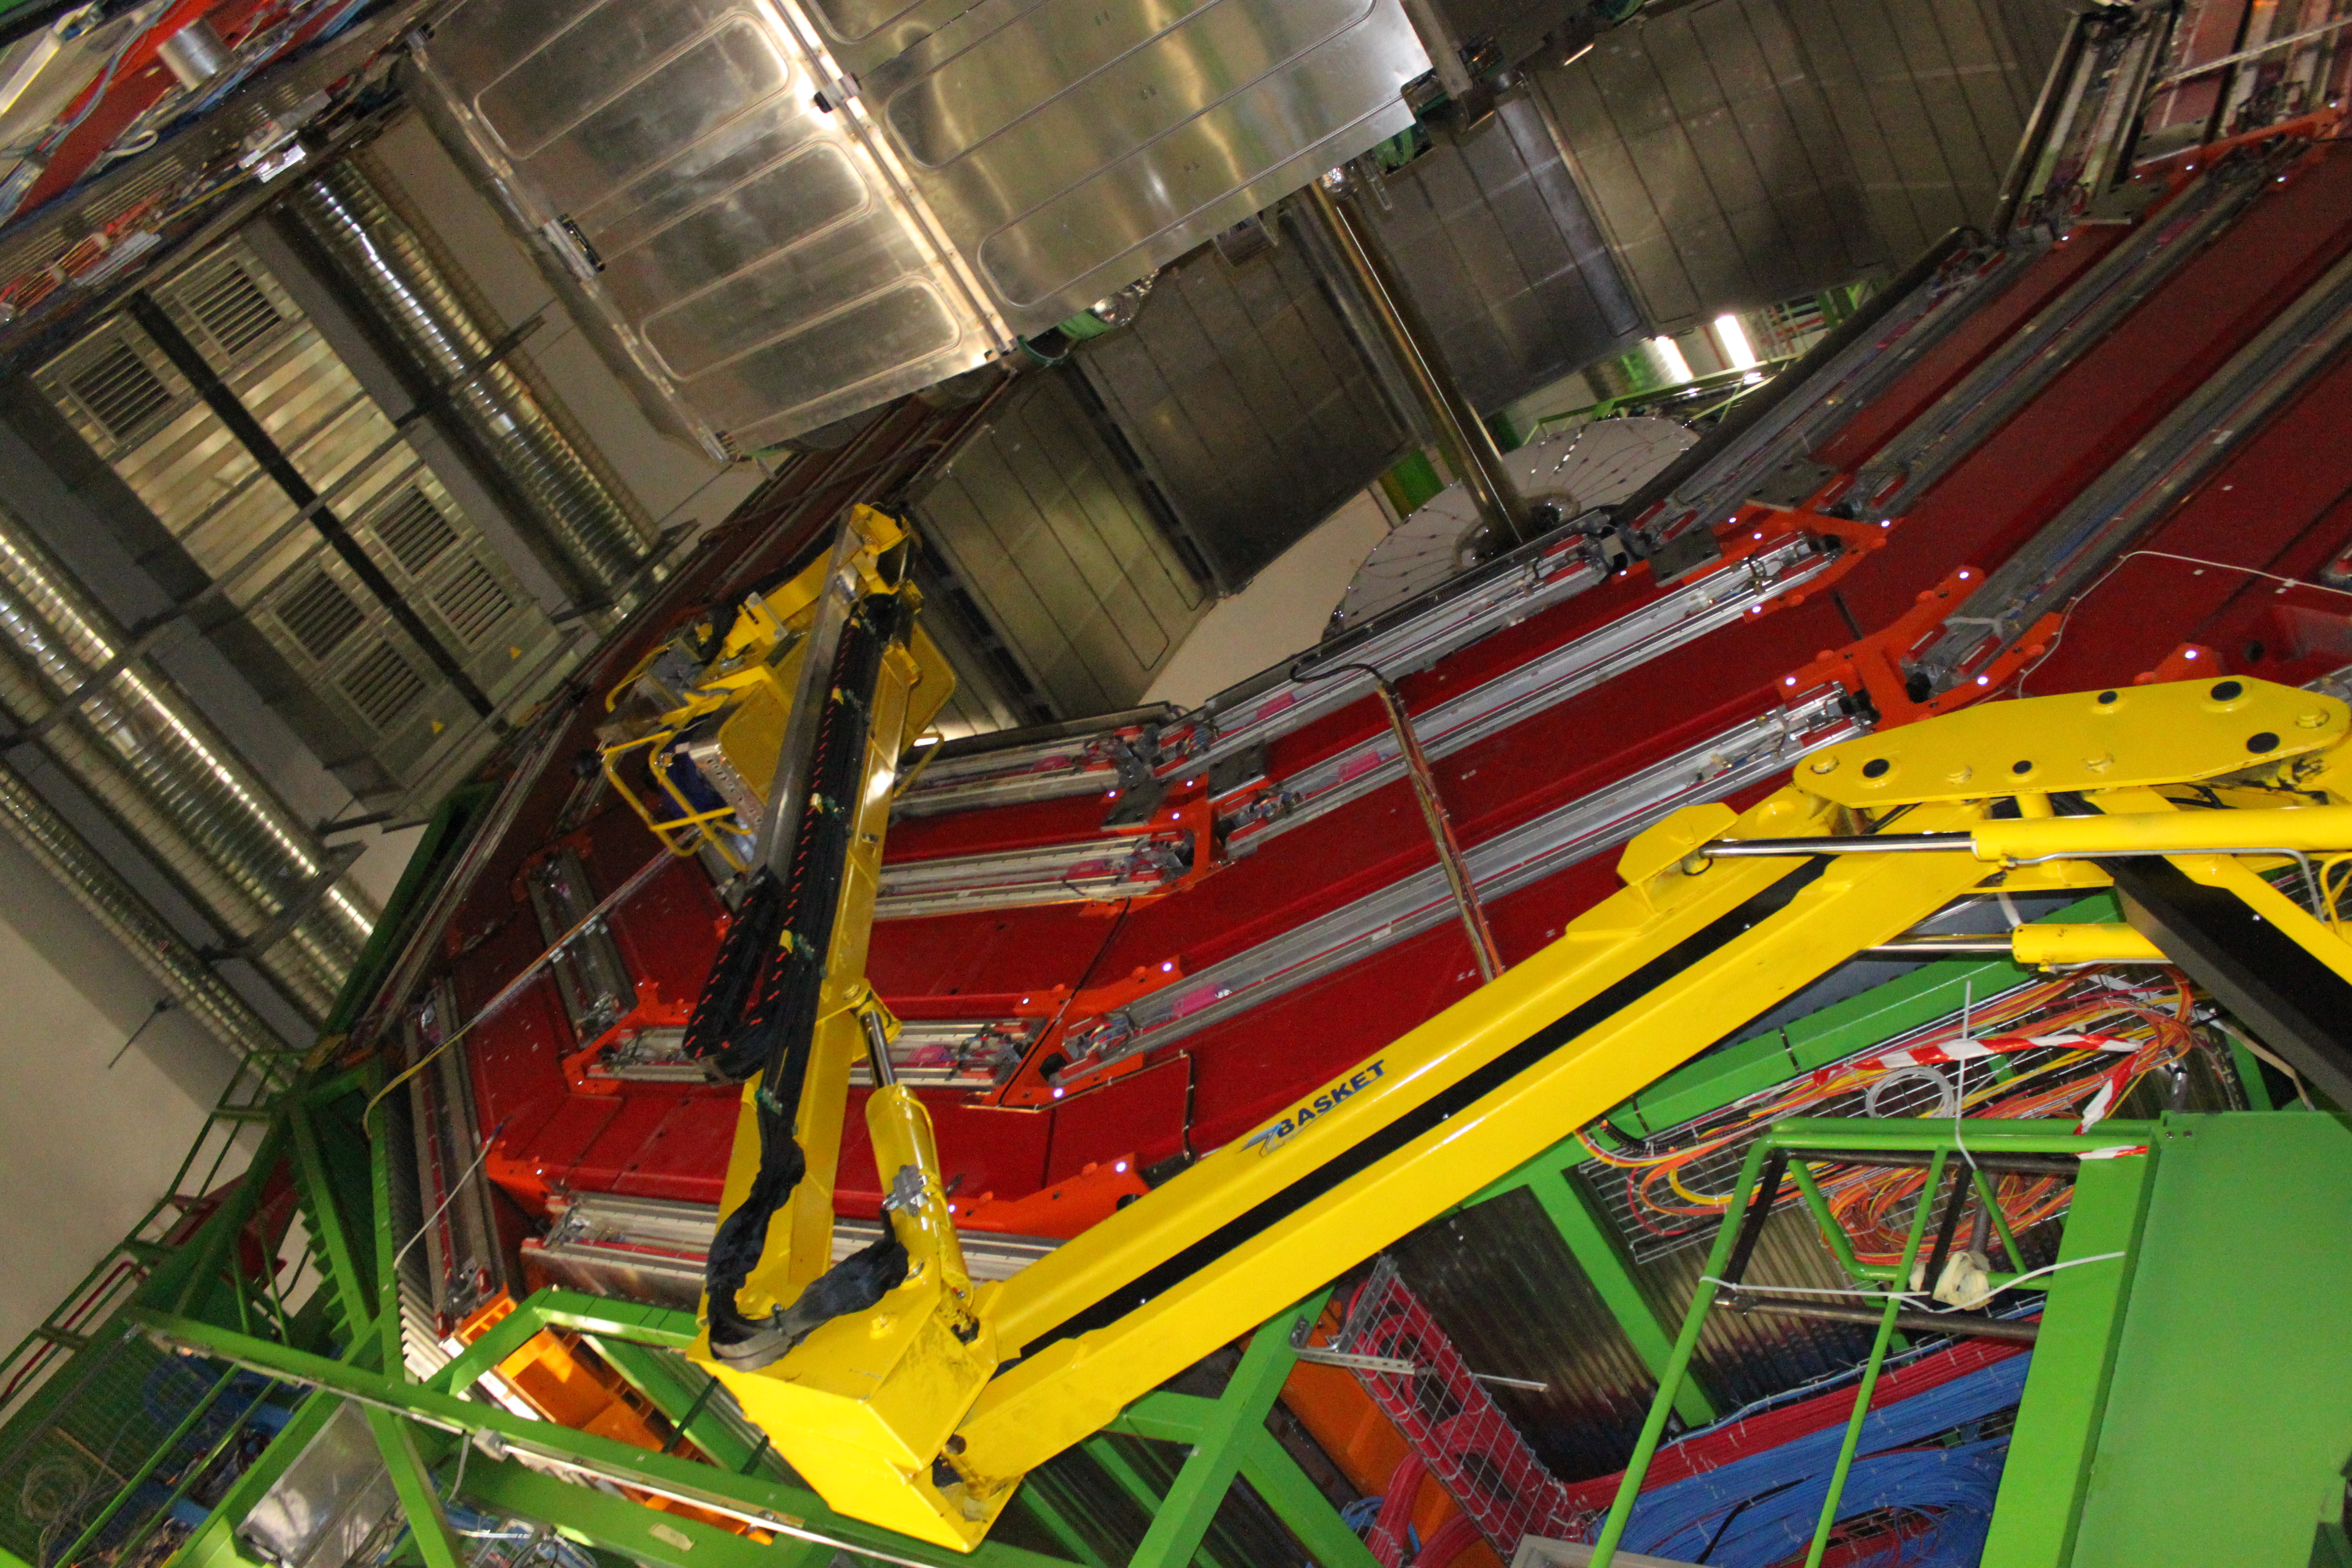
\includegraphics[width=.40\linewidth]{CMS/HO.jpg}\label{HO}}
%http://cms.desy.de/e53612/e155171/e155181/
\subfloat[Un des HF du HCAL.]{\includegraphics[width=.40\linewidth]{CMS/HF.jpg}\label{HF}}
\caption{Photos des différents composants du calorimètre hadronique.}
\end{figure}
\vspace*{-0.3cm}	
\subsection{L'aimant supraconducteur}
\vspace*{-0.3cm}
L'aimant supraconducteur de CMS (cf.Fig~\ref{MAGNET}) est un solénoïde de \SI{5.9}{\meter} de diamètre pour \SI{12.9}{\meter} de longueur qui a été prévu pour créer un champ magnétique de \SI{4}{\tesla} à un courant de \SI{19.14}{\kilo\ampere}. À pleine puissance, il stocke une énergie de \SI{2.7}{\giga\joule}. Il est composé de \num{5} bobines en nobium-titane composées de \num{2168} spires, refroidies à une température de \SI{4.2}{\kelvin} par de l'hélium liquide. Une structure de retour de champ en fer de \num{11500} tonnes, composée de \num{5} culasses (cf.Fig~\ref{CULASSE}) et \num{2} bouchons, chacun composé de \num{3} disques, l'entoure et sert de structure de maintien des chambres à muons. L'épaisseur totale du retour est d'environ \SI{1.5}{\meter} (l'épaisseur du troisième disque des bouchons et du premier anneau du tonneau est de \SI{30}{\centi\meter}) et les autres disques des bouchons ainsi que les deuxième et troisième anneaux du tonneau font \SI{60}{\centi\meter}. L'épaisseur à été étudiée afin d'être suffisante pour absorber les hadrons qui traverseraient les calorimètres et l'aimant tout en restant assez fin pour éviter les pertes radiatives pour les muons.
\marginpar
{
	\centering
	\includegraphics[width=\marginparwidth]{CMS/CULASSE.jpg}
	\captionof{figure}{Photo d'une culasse.}
	\label{CULASSE}
}
\begin{figure}[ht!]
	\centering
	\includegraphics[width=0.50\textwidth]{CMS/MAGNET.png}
	\captionof{figure}{Schéma de l'aimant supra-conducteur de CMS.}
	\label{MAGNET}
\end{figure}
\newpage
La figure \ref{CHAMP} montre une simulation par éléments-finis de la valeur du champ magnétique en fonction de la position.
\begin{figure}[ht!]
	\centering
	\includegraphics[width=0.90\textwidth]{CMS/CHAMP.png}
	\captionof{figure}{Valeur du champ magnétique (gauche) et lignes de champ (droite) selon une coupe longitudinale du détecteur CMS, prédits par la simulation. Pour une valeur du champ central de \SI{3.8}{\tesla}.}
	\label{CHAMP}
\end{figure}
\subsection{Le spectrographe à muons}
\label{RPCPRE}
Le spectographe à muons (cf.Fig~\ref{CMS1}, Fig.~\ref{CMS2}) a pour but d'identifier les muons, de mesurer avec précision leur quantité de mouvement et de déclencher sur les événements contenant des muons.
\marginpar
{
	\centering
	\includegraphics[width=\marginparwidth]{CMS/MUON.png}
	\captionof{figure}{Quart d'une coupe dans le plan transverse du détecteur CMS montrant la trajectoire d'un muon (courbe bleue).}
	\label{MUON}
} Les muons ont un très grand pouvoir de pénétration. Il est donc possible d'utiliser à la fois les traces chargées laissées dans le trajectographe et dans des détecteurs placés après l'aimant pour les identifier et les reconstruire de manière précise. Une bonne résolution de la quantité de mouvement des muons et leur bonne identification est obtenue grâce au champ magnétique intense de l'aimant et du retour de champ dans la culasse qui assure une trajectoire avec une double courbure. Cette culasse doit contenir des détecteurs de grande taille afin d'augmenter la probabilité de détection. Ils faut donc qu'ils soient peu onéreux et fiables. Il faut également que ces détecteurs ne soient pas atteints par d'autres particules afin d'assurer un signal propre, pour ce faire la distance depuis l'aimant jusqu'à la dernière station du spectrographe et de l'ordre de \num{16} longueurs de radiation, ce qui évite le bruit de fond hadronique résiduel venant du faisceau.

\begin{sidewaysfigure}
\centering
\includegraphics[width=0.80\textwidth]{CMS/CMSLONG.png}
\captionof{figure}{Coupe longitudinale d'un quart de CMS.}
\label{CMS1}
\end{sidewaysfigure}


\begin{figure}[p]
\centering
\includegraphics[width=0.98\textwidth]{CMS/CMSTRANS.png}
\captionof{figure}{Coupe transversale de la partie centrale CMS.}
\label{CMS2}
\end{figure}

Le spectrographe à muons, est composé de \num{3} sous-détecteurs :
\begin{itemize}[label=$\bullet$]
	\item \textbf{Les chambres à dérive} DT pour \textit{Drift Tube} (cf.Fig~\ref{DT}) sont présentes seulement dans le tonneau où le flux de muons est faible tout comme le bruit de fond des neutrons. Le champ magnétique est également assez faible ($\sim$\SI{0.4}{\tesla}) et uniforme. Ce détecteur est constitué de \num{250} chambres insérées dans la culasse de CMS. Elles sont disposées en quatre couches selon $r$ à des distances $r=$\num{4.0}, \num{4.9}, \num{5.9} et \SI{7.0}{\meter}. La culasse est composée selon l'axe $z$ de \num{5} roues numérotées de $-$\num{2} à \num{2}, chacune comportant \num{12} (sauf pour MB4 qui en possède \num{14} (cf.Fig~\ref{CMS2})) secteurs dans le plan transverse numérotés à partir de $\phi=$\num{0} et couvrant \SI{30}{\degree}. Ce détecteur couvre une zone en pseudo rapidité $|\eta|<$\num{1.2}. Chaque chambre est constituée de \num{8} couches de tubes (cf.Fig~\ref{DT1}) mesurant la courbure de la trajectoire des muons selon $\phi$ et \num{4} couches pour la courbure selon $\eta$. Chaque ensemble de \num{4} couches est appelé super-couche (\textit{superlayer}). Les deux super-couches mesurant $\phi$ sont séparées par \SI{20}{\centi\meter} d'aluminium en nid d'abeilles. Seules les chambres de MB4 ne possèdent pas de \textit{superlayer} mesurant $\eta$ bien que la distance entre les deux \textit{superlayers} reste la même.
	\begin{figure}[ht!]
		\centering
		\includegraphics[width=0.40\textwidth]{CMS/DTchamber.png}
		\captionof{figure}{Schéma d'une chambre à dérive.}
		\label{DT1}
	\end{figure}

    Les tubes d'une couche de la chambre sont constitués de \num{5} électrodes : un fil d'acier inoxydable au centre du tube composant l'anode, \num{2} pistes servant de cathodes et \num{2} pistes servant d'électrodes et à mettre en forme le champ électrique. Ces deux électrodes améliorent l'uniformité du champ à l'intérieur du tube loin du fil et améliorent ainsi la résolution spatiale. Le tube est rempli d'un gaz de \chemform{ArCO_2} \num{85}/\num{15}. Lorsqu'une particule traverse le tube, elle ionise le gaz qui libère des électrons qui sont ensuite accélérés vers l'anode. Une avalanche se crée près du fil, où le champ électrique est intense, ce qui induit un signal sur le fil. Le temps de dérive est d'environs \SI{380}{\nano\second}. 
    
    	\begin{figure}[ht!]
    	\centering
    	\includegraphics[width=0.45\textwidth]{CMS/DTTUBE.png}
    	\captionof{figure}{Schéma d'un tube d'une chambre à dérive.}
    	\label{DT2}
    	\end{figure}
    En estimant le temps d'arrivée des électrons sur l'anode, en supposant le temps d'interaction connu et en ayant trois couches d'un superlayer touchées, il est possible d'estimer la position et le temps de la trace. Dans un superlayer une résolution de \SI{20}{\milli\radian} en angle, de \SI{100}{\micro\meter} en position et de quelques \si{\nano\second} en temps est atteinte.
    
    \item \textbf{Les chambres à pistes cathodiques} CSC pour \textit{Cathode Strip Chambers} (cf.Fig~\ref{CSC}) sont présentes dans les bouchons où le flux de muons ainsi que le bruit de fond sont importants, le champ magnétique est également non-uniforme. Ces chambres ont un temps de réponse très court, une granularité fine et sont presque insensibles à la non-uniformité du champ magnétique. Ce détecteur couvre les zones de pseudo-rapidité \num{0.9}$<=|\eta|<=$\num{2.4} et consiste en \num{468} chambres installées dans les bouchons. Chaque bouchon comprend \num{4} stations nommées ME1, ME2, ME3 et ME4. Chaque station comprend \num{2} anneaux (sauf ME1 qui en comprend \num{3}) segmentés en \num{36} chambres couvrant chacune un angle de \SI{10}{\degree} en $\phi$.
    
    Les chambres (cf.Fig~\ref{CSC2}) sont constituées de \num{6} couches contenant un mélange de gaz (\num{40}\% \chemform{Ar} \num{50}\% \chemform{CO_2} qui assure un bon gain et \num{10}\% \chemform{CF_4} afin d'empêcher la polymérisation près des fils.) ainsi qu'un plan de pistes de cathodes radiales et de fils séparés de \SI{3}{\milli\meter} constituant les anodes placées orthogonalement aux pistes (sauf pour les premier anneaux de ME1 ou les fils sont orientés à \SI{26}{\degree} afin de compenser la force de \bsc{Lorentz} due au champ magnétique de \SI{4}{\tesla} dans cette zone). Le nombre total de pistes est de \num{220 000} pour plus de \num {2 000 000} fils.
    
    Lorsqu'une particule chargée traverse une CSC, elle ionise le gaz. Les électrons sont accélérés vers le fils d'anode. Le mouvement de ces charges induit un signal sur les pistes cathodes et les fils anodes de la chambre. Le temps de dérive est beaucoup plus rapide que pour les DT mais la résolution spatiale est plus faible : \SI{150}{\micro\meter} dans le plan transverse.
    \begin{figure}[ht!]
    	\centering
    	\includegraphics[width=0.60\textwidth]{CMS/CSC2.png}
    	\captionof{figure}{Schéma d'une chambre CSC.}
    	\label{CSC2}
    \end{figure}
    
	\item \textbf{Les chambres à plaques résistives} ou \textit{Resistive Plate Chambers} (RPC) (cf.Fig~\ref{RPC}) forment un système très efficace pour déclencher sur les muons même à bas $p_{T}$ et sur une zone en pseudo rapidité très large ($|\eta|<$\num{1.6}) grâce à son excellente résolution temporelle ($\sim$\si{\nano\second}). Elles complètent les détecteurs CSC et DT dont les résolutions spatiales sont beaucoup plus élevées. Les RPC permettent d'assigner avec une plus grande précision le bon temps de croisement de faisceau pour les muons. Elles sont présentes à la fois dans le tonneau et les bouchons. Dans le tonneau \num{480} sont réparties en \num{6} couches, \num{2} pour MB1 et MB2 et \num{1} pour MB3 et MB4. La redondance en MB1 et MB2 permet de déclencher sur les muons de bas $p_{T}$ qui pourraient être arrêtés avant d'atteindre MB3. Pour les bouchons, les \num{432} chambres sont répartis en trois disques noté RE1, RE2 et RE3 pour chaque bouchon. Chaque disque est composé de \num{3} anneaux RE*/1 RE*/2 RE*/3 avec * représentant le numéro du disque. Seuls les anneaux \num{2} et \num{3} sont instrumentés. Chaque anneaux est segmenté en \num{36} chambres couvrant $\phi=$\SI{10}{\degree}.
	
	Les RPC sont des chambres à double \textit{gaps} (cf.Fig~\ref{RPC2}) qui opèrent en mode avalanche afin de fonctionner même à haut flux de particules $\sim$\SI{100}{\hertz\per\square\centi\meter}. Un gap est constitué de deux plaques de bakélite qui servent d'électrodes entres lesquelles circule un gaz. Des pistes de lecture sont insérées entre les deux gaps. Le système des RPC dans CMS ainsi que le fonctionnement d'une RPC sont expliqués dans le prochain chapitre.
	
	  \begin{figure}[ht!]
		\centering
		\includegraphics[width=0.80\textwidth]{CMS/RPC2.jpg}
		\captionof{figure}{Schéma en vue éclatée d'un gap d'une RPC et des pistes de lecture.}
		\label{RPC2}
	\end{figure}
	
	
\end{itemize}
    \begin{figure}[ht!]
	\centering
	\subfloat[Une cassette contenant une chambre DT et RPC.]{\includegraphics[width=0.40\linewidth]{CMS/DT.jpg}\label{DT}}
	\subfloat[Une chambre CSC.]{\includegraphics[width=.40\linewidth]{CMS/CSC.jpg}\label{CSC}}
	\\
	\subfloat[Une chambre RPC.]{\includegraphics[width=.40\linewidth]{CMS/RPC.jpg}\label{RPC}}
	\caption{Photos des différents composants du spectrographe à muons.}
\end{figure}

\section{Le système de déclenchement et d'acquisition de données}
Chaque type de particules lors de son passage dans CMS va créer des types de traces particulières qui vont être enregistrées sous forme électronique par les sous-détecteurs le composant. La figure \ref{particules} montre une vue schématique des traces laissées par différents types de particules dans les sous-détecteurs de CMS.

	  \begin{figure}[ht!]
	\centering
	\includegraphics[width=0.52\textwidth]{CMS/particles.png}
	\captionof{figure}{Schéma des traces laissées par différents types de particules dans les sous détecteurs de CMS.}
	\label{particules}
\end{figure}

Les faisceaux ont une fréquence de croisement de \SI{40}{\mega\hertz}, chaque événement créé lors de ces collisions génère environ un Méga-octets de données. Le flux de données est bien trop important pour être stocké ($\sim$\SI{40}{\tera\byte\per\second}). Celui-ci doit donc être réduit, il est donc nécessaire de rejeter des événements afin d'obtenir une fréquence d'acquisition de l'ordre de \SI{300}{\hertz} tout en continuant d'enregistrer les événements intéressants pour la physique. Cette étape est réalisée par le système de déclenchement ou \textit{trigger}. La réduction d'un facteur \num{e5} du taux d'acquisition des données est impossible à réaliser en une seule fois, le \textit{trigger} est donc constitué de deux étapes appelées \textit{Level-1 Trigger} (L1) qui réduit le flux d'événements à \SI{100}{\kilo\hertz} et \textit{High-Level Trigger} (HLT) qui réduit ensuite ce flux à \SI{300}{\hertz}.

\subsection{Le déclenchement de niveau I (L1)}
Le trigger de niveau I (L1) (cf.Fig~ \ref{L1}) opère à la fréquence de collision des faisceaux (\SI{40}{\mega\hertz}). L'électronique des détecteurs lit et stocke les  signaux électriques dans une mémoire tampon de \num{128} événements de collisions soit \SI{3.2}{\micro\second}. Le système de déclenchement possède donc \SI{3.2}{\micro\second} pour  décider s'il doit envoyer les données au déclenchement de haut niveau HLT. Chaque \SI{25}{\nano\second}, un nouvel événement rentre dans la mémoire tampon et la décision de garder ou non l'événement arrivé \SI{3.2}{\micro\second} plus tôt est prise. Les \SI{3.2}{\micro\second} correspondent à l'envoi des données depuis l'électronique des calorimètres et du spectrographe à muons vers la caverne de services qui contient les processeurs gérant la prise de décision, le retour d'un signal pour le rejet ou l'acceptation de l'événement, le délai de synchronisation entre les parties du détecteur ainsi que le temps de prise de décision en lui-même ($\sim$\SI{1}{\micro\second}). 

	  \begin{figure}[ht!]
	\centering
	\includegraphics[width=0.70\textwidth]{CMS/L1.png}
	\captionof{figure}{Schéma du Level-1 Trigger (L1).}
	\label{L1}
\end{figure}

Chacun des trois sous-détecteurs du spectrographe à muons utilise son propre système de déclenchement. Les DT et CSC créent des segments de traces. Ces segments ne sont conservés que s'il pointent vers le point d'interaction. Deux (trois) traces par DT (CSC) sont envoyées au \textit{Drift Tube Track Finder} (DTTF) (\textit{Cathode Strip Chamber Track Finder }(CSCTF)) qui cherchent des correspondances entre les traces et assignent un niveau de qualité aux valeurs $\eta$, $\phi$, à la charge et à la quantité de mouvement trouvées par ces correspondances. Quatre candidats muons sont envoyés au \textit{Global Muon Trigger} (GMT) par les \textit{"Finder"}. Pour les RPC, la sélection est basée sur une coïncidence spatiale et temporelle entre les différentes couches. Le \textit{Pattern Comparator} compare les signaux venant des \num{4} stations à des patrons prédéfinis afin de trouver les candidats muons et \num{8} d'entre eux (\num{4} pour les bouchons \num{4} pour le tonneau) sont envoyés au GMT. Le GMT reçoit tous ces candidats et combine ceux trouvés dans plusieurs sous-detecteurs. Il assigne ensuite un niveau de qualité à ces nouveaux candidats et envoie les \num{4} meilleurs d'entre eux au \textit{Global Trigger} (GT).

Les calorimètres sont réunis en tours de déclenchement qui correspondent aux super-cristaux pour le ECAL. Un candidat est trouvé pour chaque tour du ECAL et HCAL. Le \textit{Trigger Primitive Generator} est responsable de sommer les énergies venant des différents composants des tours.  Le \textit{Regional Calorimeter Trigger} (RCT) reçoit les candidats du ECAL et HCAL qui sont répartis en \num{18} \textit{crates} qui couvrent la moitié des détecteurs en $z$ et \SI{40}{\degree} en $\phi$ et fournissent au \textit{Global Calorimeter Trigger} chacun \num{4} candidats $e/\gamma$ isolés et \num{4} candidats non-isolés. Le GCT fournit des informations sur l'isolation et la compatibilité avec des particules d'ionisation minimale au système \textit{trigger} des muons et classe les candidats $e/\gamma$ par niveau de qualité et envoie les \num{4} meilleurs isolés et les \num{4} meilleurs non-isolés au GT. Le GT possède également des informations sur les jets, l'énergie transverse totale, etc.

La décision finale est faite par le \textit{Global Trigger} à partir de conditions programmables demandant la présence d'objets ou d'énergie en quantité ou valeurs prédéfinies. Ces conditions forment un chemin de déclenchement. Le \textit{Global Trigger} permet de programmer et de tester jusqu'à \num{128} chemins en parallèle. 

\subsection{Le déclenchement de haut niveau (HLT)}
Si l'événement est sélectionné par le L1, il est envoyé au déclenchement de haut niveau (HLT) et les données sont transmises à une ferme de calcul de plusieurs milliers d'ordinateurs  dont chaque processeur exécute le même code de déclenchement (\textit{HLT Menu}) séquentiellement afin de réduire le temps nécessaire à l'élimination d'un événement et d'améliorer le temps de décision qui doit être de l'ordre de \SI{100}{\milli\second} par événement. Il permet de passer à un flux de donnée de \SI{300}{\hertz}. Durant cette phase, les données du \textit{tracker} sont utilisées contrairement au L1.

\section{Mises à niveau et amélioration de CMS}
Le détecteur CMS à déjà subi de nombreuses améliorations depuis le début de sa mise en service (SiPM dans le HO, nouveau trajectographe à pixels\ldots). Cependant, la mise à niveau du LHC vers le HL-LHC prévoit de multiplier la luminosité par \num{7.5}, ce qui représente un défi pour CMS qui doit se mettre à niveau pendant les arrêts LS2 et LS3 afin de pouvoir s'adapter à cette luminosité et au \textit{pile-up} supplémentaire que cela va engendrer ($\sim$\num{140}--\num{200} événements de \textit{pile-up}). Parmi les mises à niveaux programmées citons \cite{Collaboration:1355706} \cite{Contardo:2020886} :
\begin{itemize}[label=$\bullet$]
	\item Le remplacement des HPD dans les sous-détecteurs HB, HE du calorimètre hadronique pendant le LS2 par des SiPM (comme actuellement dans le HO).
	\item Le remplacement complet du trajectographe durant LS3 (cf.Fig~\ref{tracker2}). La granularité doit être multipliée par \num{4} afin de garder une bonne performance de reconstruction malgré l'augmentation du \textit{pile-up}. Pour cela, les pistes du trajectographe à pistes seront raccourcies et le détecteur sera également plus léger afin d'obtenir une meilleure résolution en $p_{T}$ et une conversion des $\gamma$ plus faible. Le trajectographe à pixels aura des pixels et des senseurs plus petits afin d'améliorer la résolution du paramètre d'impact et une meilleure séparation des traces. Plus de \num{10} disques additionnels dans chaque bouchon seront installés afin de couvrir une zone en rapidité jusqu'à $|\eta|=$\num{4}.
	\begin{figure}[ht!]
		\centering
		\includegraphics[width=0.88\textwidth]{CMS/tracker2.png}
		\captionof{figure}{Schéma d'un quart du trajectographe prévu pour la mise à niveau de CMS.}
		\label{tracker2}
	\end{figure}
	\item Les bouchons des calorimètres devront être remplacés par des calorimètres de haute granularité \textit{High Granularity Calorimeter} (HGC) d'une profondeur totale de $\sim$\num{10}$\lambda_{I}$ qui fourniront des images tridimensionnelles détaillées des gerbes. La section électromagnétique est composée d'une trentaine de couches de tungstène et de plaques de cuivre intercalées avec des capteurs de silicium comme matière active. Les capteurs auront des aires variables inférieures à $\sim$\SI{1,0}{\square\centi\meter}. La section électromagnétique fait environs \num{25}$X_0$ et une longueur d'interaction ($\lambda_{I}$). La partie hadronique possède \num{12} plaques de laiton et de cuivre intercalées avec des capteurs de silicium d'une longueur représentant \num{3,5}$\lambda_{I}$ ce qui couvre la majorité d'une gerbe hadronique. Il est suivi d'un "calorimètre hadronique à l'arrière" de conception similaire à l'actuel HE (des plaques en laiton intercalées avec des carreaux scintillants en plastique lus avec des fibres optiques à décalage de longueur d'ondes). La conception de ce calorimètre à grande granularité s'appuie sur les concepts du ILC/CALICE pour la mesure 3D des gerbes.
	\item le temps de latence du L1 sera augmenté jusqu'à \SI{12.5}{\micro\second} ce qui permettra au système de reconstruction et d'identification des traces d'utiliser à la fois celles venant des calorimètres et celles du spectrographe à muons. Pour cela l'électronique de certains sous-détecteurs déjà existant devra être mise à niveau. La fréquence des données en sortie est estimée à \SI{5000}{\hertz} (\SI{7000}{\hertz}) avec \num{140} (\num{200}) événements de \textit{pile-up}. Le trigger L1 aura également les informations des traces fournies par le trajectographe pour des traces avec $p_{T}\geq$\SI{2}{\giga\eV}. Cela permettra un meilleur pouvoir de rejet du bruit de fond dès le début de la sélection des événements. Un tout nouveau L1 pour les calorimètres et le spectrographe à muons sera également mis en service (cf.Fig~\ref{L1_2}).
	\begin{figure}[ht!]
		\centering
		\includegraphics[width=0.55\textwidth]{CMS/L1_2.png}
		\captionof{figure}{Schéma du nouveau L1 pour la partie calorimètre et muons.}
		\label{L1_2}
	\end{figure}
\item Le trajectographe à muons dans les bouchons ne possède actuellement que des CSC dans la zone \num{1.6}$<|\eta|<$\num{2.4}. C'est la seule région du trajectographe qui ne possède pas de RPC afin d'assurer une redondance malgré le fait qu'il s'agisse d'une région dont la résolution de la quantité de mouvement est moins bonne et dont le bruit de fond est important. Afin d'améliorer le L1 dans cette région il est proposé d'instrumenter cette zone avec des chambres de nouvelle technologie. Il est donc prévu d'utiliser des \textit{Gas Electron Multiplier} (GEM) dans les stations ME1 et ME2 qui présentent une bonne résolution spatiale et qui résistent au champ magnétique important présent dans ces zones. Elles permettront d'améliorer la résolution en quantité de mouvement et d'améliorer la correspondance avec les traces dans le \textit{Global Muon Trigger}. Pour les deux dernières zones ME3 et ME4, des RPC de meilleure granularité et de bonne résolution temporelle seront utilisés afin de réduire le bruit de fond.  De plus, une nouvelle station ME0 de GEM sera insérée dans l'espace libéré par les nouveaux bouchons de CMS, ce qui augmentera la couverture de détection des muons jusqu'à $|\eta|\approx$\num{3} (cf.Fig~\ref{end}). 
	\begin{figure}[ht!]
	\centering
	\includegraphics[width=0.60\textwidth]{CMS/endcap.png}
	\captionof{figure}{Schéma d'un quart du détecteur CMS montrant les différentes technologies qui seront utilisées dans les bouchons du spectrographe à muons.}
	\label{end}
\end{figure}
\end{itemize}
Ce dernier point et plus particulièrement la caractérisation de détecteurs à plaques résistives de verres de basse résistivité est l'objet de cette thèse et sera développé dans les chapitres suivants.